% include the figures path relative to the master file
\graphicspath{ {./content/other/figures/} }

\section{PARTS OF MANUSCRIPT} 

This section describes the normal structure of a manuscript and how each part should be handled.  The appropriate vertical spacing between various parts of this document is achieved in LaTeX through the proper use of defined constructs, such as \verb|\section{}|.  In LaTeX, paragraphs are separated by blank lines in the source file. 

At times it may be desired, for formatting reasons, to break a line without starting a new paragraph.  This situation may occur, for example, when formatting the article title, author information, or section headings.  Line breaks are inserted in LaTeX by entering \verb|\\| or \verb|\linebreak| in the LaTeX source file at the desired location.  

%%%%%Sometimes it is necessary to precede the double slash 
%%%%%by \verb|\protect| to get the desired result, 
%%%%%for example, in article titles.

%%-----------------------------------------------------------
\subsection{Title and Author Information} 
\label{sec:title}

The article title appears centered at the top of the first page.  The title font is 16 point, bold.  The rules for capitalizing the title are the same as for sentences; only the first word, proper nouns, and acronyms should be capitalized.  Avoid using acronyms in the title.  Keep in mind that people outside your area of expertise might read your article.  Appendix~\ref{sec:misc} contains more about acronyms.

The list of authors immediately follows the title after a blank vertical space of about 7 mm.  The font is 12 point, normal with each line centered.  The authors' affiliations and addresses follow the author list after another blank space of about 4 mm, also in 12-point, normal font and centered.  Do not use acronyms in affiliations and addresses. For multiple affiliations, each affiliation should appear on a new line, separated from the following address by a semicolon.  Italicized superscripts may be used to identify the correspondence between the authors and their respective affiliations.  Further author information, such as e-mail address, complete postal address, and web-site location, may be provided in a footnote by using \verb|\authorinfo{}|, as demonstrated above.

When the abbreviated title or author information is too long to fit on one line, multiple lines may be used; insert line breaks appropriately to achieve a visually pleasing format.  The proper spacing of one and one-half lines between the title, author list, and their affiliations is achieved with the command \verb|\skiplinehalf| defined in {\tt spie.cls}.

%%-----------------------------------------------------------
\subsection{Abstract and Keywords} 
The title and author information is immediately followed by the Abstract. The Abstract should concisely summarize the key findings of the paper.  It should consist of a single paragraph containing no more than 200 words.  The Abstract does not have a section number.  A list of up to ten keywords should immediately follow the Abstract after a blank line.  These keywords will be included in a searchable database at SPIE.

%%-----------------------------------------------------------
\subsection{Body of Paper} 
The body of the paper consists of numbered sections that present the main findings.  These sections should be organized to best present the material.  See Sec.~\ref{sec:sections} for formatting instructions.

%%-----------------------------------------------------------
\subsection{Appendices} 
Auxiliary material that is best left out of the main body of the paper, for example, derivations of equations, proofs of theorems, and details of algorithms, may be included in appendices.  Appendices are enumerated with uppercase Latin letters in alphabetic order, and appear just before the Acknowledgments and References.

%%-----------------------------------------------------------
\subsection{Acknowledgments} 
In the Acknowledgments section, appearing just before the References, the authors may credit others for their guidance or help.  Also, funding sources may be stated.  The Acknowledgments section does not have a section number.

%%-----------------------------------------------------------
\subsection{References} 
The References section lists books, articles, and reports that are cited in the paper.  It does not have a section number.  The references are numbered in the order in which they are cited.  Examples of the format to be followed are given at the end of this document.  

The reference list at the end of this document is created using BibTeX, which looks through the file {\tt report.bib} for the entries cited in the LaTeX source file.  The format of the reference list is determined by the bibliography style file {\tt spiebib.bst}, as specified in the \verb|\bibliographystyle{spiebib}| command.  Alternatively, the references may be directly formatted in the LaTeX source file.

For books\cite{Lamport94,Alred03,Goossens97} the listing includes the list of authors, book title (in italics), page or chapter numbers, publisher, city, and year of publication.  A reference to a journal article\cite{Metropolis53} includes the author list, title of the article (in quotes), journal name (in italics, properly abbreviated), volume number (in bold), inclusive page numbers, and year.  By convention\cite{Lamport94}, article titles are capitalized as described in Sec.~\ref{sec:title}.  A reference to a proceedings paper or a chapter in an edited book\cite{Gull89a} includes the author list, title of the article (in quotes), conference name (in italics), if appropriate, editors, volume or series title (in italics), volume number (in bold), if applicable, inclusive page numbers, publisher, city, and year.  References to an article in the SPIE Proceedings may include the conference name, as shown in Ref.~\citenum{Hanson93c}.

Citations to the references are made using superscript numerals, as demonstrated in the preceding paragraph.  One may also directly refer to a reference within the text, e.g., ``as shown in Ref.~\citenum{Metropolis53} ..." 

%%-----------------------------------------------------------
\subsection{Footnotes} 
Footnotes\footnote{Footnotes are indicated as superscript symbols to avoid confusion with citations.} may be used to provide auxiliary information that doesn't need to appear in the text, e.g., to explain measurement units.  They should be used sparingly, however.  

Only nine footnote symbols are available in LaTeX. If you have more than nine footnotes, you will need to restart the sequence using the command  \verb|\footnote[1]{Your footnote text goes here.}|. If you don't, LaTeX will provide the error message {\tt Counter too large.}, followed by the offending footnote command.

%%%%%%%%%%%%%%%%%%%%%%%%%%%%%%%%%%%%%%%%%%%%%%%%%%%%%%%%%%%%%
\section{SECTION FORMATTING} \label{sec:sections}

Section headings are centered and formatted completely in uppercase 11-point bold font.  Sections should be numbered sequentially, starting with the first section after the Abstract.  The heading starts with the section number, followed by a period.  In LaTeX, a new section is created with the \verb|\section{}| command, which automatically numbers the sections.

Paragraphs that immediately follow a section heading are leading paragraphs and should not be indented, according to standard publishing style\cite{Lamport94}.  The same goes for leading paragraphs of subsections and sub-subsections.  Subsequent paragraphs are standard paragraphs, with 14-pt.\ (5 mm) indentation.  An extra half-line space should be inserted between paragraphs.  In LaTeX, this spacing is specified by the parameter \verb|\parskip|, which is set in {\tt spie.cls}.  Indentation of the first line of a paragraph may be avoided by starting it with \verb|\noindent|.
 
%%-----------------------------------------------------------
\subsection{Subsection Attributes} 

The subsection heading is left justified and set in 11-point, bold font.  Capitalization rules are the same as those for book titles.  The first word of a subsection heading is capitalized.  The remaining words are also capitalized, except for minor words with fewer than four letters, such as articles (a, an, and the), short prepositions (of, at, by, for, in, etc.), and short conjunctions (and, or, as, but, etc.).  Subsection numbers consist of the section number, followed by a period, and the subsection number within that section.  

%%-----------
\subsubsection{Sub-subsection attributes} 
The sub-subsection heading is left justified and its font is 10 point, bold.  Capitalize as for sentences.  The first word of a sub-subsection heading is capitalized.  The rest of the heading is not capitalized, except for acronyms and proper names.  

%%%%%%%%%%%%%%%%%%%%%%%%%%%%%%%%%%%%%%%%%%%%%%%%%%%%%%%%%%%%%
\section{FIGURES AND TABLES} 

Figures are numbered in the order of their first citation.  They should appear in numerical order and on or after the same page as their first reference in the text.  Alternatively, all figures may be placed at the end of the manuscript, that is, after the Reference section.  It is preferable to have figures appear at the top or bottom of the page.  Figures, along with their captions, should be separated from the main text by at least 0.2 in.\ or 5 mm.  

Figure captions are centered below the figure or graph.  Figure captions start with the figure number in 9-point bold font, followed by a period; the text is in 9-point normal font; for example, ``{\footnotesize{Figure 3.}  Original image...}".  See Fig.~\ref{fig:example} for an example of a figure caption.  When the caption is too long to fit on one line, it should be justified to the right and left margins of the body of the text.  

Tables are handled identically to figures, except that their captions appear above the table. 
%%  Use following command to specify that graphics file is in 
%%  a directory other than this LaTeX source file.
%%  Note use of / to separate subdirectories, for UNIX and Windows OS.
%%\graphicspath{{H:/HANSON/SPIESTY/}}
%% tabular environment useful for creating an array of images  
%-------------
   \begin{figure}
   \begin{center}
   \begin{tabular}{c}
   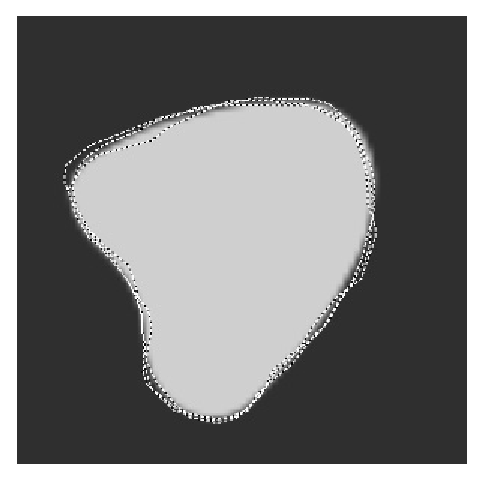
\includegraphics[height=7cm]{mcr3b.eps}
   \end{tabular}
   \end{center}
   \caption[example] 
%>>>> use \label inside caption to get Fig. number with \ref{}
   { \label{fig:example} 
Figure captions are used to describe the figure and help the reader understand it's significance.  The caption should be centered underneath the figure and set in 9-point font.  It is preferable for figures and tables to be placed at the top or bottom of the page. LaTeX tends to adhere to this standard.}
   \end{figure} 
%-------------

For further details concerning the inclusion of grayscale and color images, consult SPIE's {\it Author Guide for Publication and Presentation}.
 
%%%%%%%%%%%%%%%%%%%%%%%%%%%%%%%%%%%%%%%%%%%%%%%%%%%%
\appendix    %>>>> this command starts appendixes
%%%%%%%%%%%%%%%%%%%%%%%%%%%%%%%%%%%%%%%%%%%%%%%%%%%%
\section{MISCELLANEOUS FORMATTING DETAILS} \label{sec:misc}

It is often useful to refer back (or forward) to other sections in the article.  Such references are made by section number.  When a section reference starts a sentence, Section is spelled out; otherwise use its abbreviation, for example, ``In Sec.~2 we showed..." or ``Section~2.1 contained a description...".  References to figures, tables, and theorems are handled the same way.

At the first occurrence of an acronym, spell it out, followed by the acronym in parentheses, e.g., noise power spectrum (NPS).  
 
%%-----------------------------------------------
\subsection{Formatting Equations} 
Equations may appear in line with the text, if they are simple, short, and not of major importance; e.g., $\beta = b/r$.  Important equations appear on their own line.  Such equations are centered.  For example, ``The expression for the minus-log-posterior is
	\begin{equation}
	\label{eq:alpha}
\phi = |{\rm\bf y} - {\rm\bf A}{\rm\bf x}|^2 + \alpha \log p({\rm\bf x}) \, ,
	\end{equation}
where $\alpha$ determines the strength of ..."  Principal equations are numbered, with the equation number placed within parentheses and right justified.  

Equations are considered to be part of a sentence and should be punctuated accordingly. In the above example, a comma follows the equation because the next line is a subordinate clause.  If the equation ends the sentence, a period should follow the equation.  The line following an equation should not be indented unless it is meant to start a new paragraph.  Indentation after an equation is avoided in LaTeX by not leaving a blank line between the equation and the subsequent text.

References to equations include the equation number in parentheses, for example, ``Equation~(\ref{eq:alpha}) shows ..." or ``Combining Eqs.~(2) and (3), we obtain..."  Using a tilde in the LaTeX source file between two characters avoids unwanted line breaks.

%%-----------------------------------------------------------
\subsection{Formatting Theorems} 

To include theorems in a formal way, the theorem identification should appear in a 10-point, bold font, left justified and followed by a period.  The text of the theorem continues on the same line in normal, 10-point font.  For example, 

\noindent{\bf Theorem 1.} For any unbiased estimator...

Formal statements of lemmas and algorithms receive a similar treatment.

%%%%%%%%%%%%%%%%%%%%%%%%%%%%%%%%%%%%%%%%%%%%%%%%%%%%
\section{SOME LATEX GUIDANCE} \label{sec:latex}

%%-----------------------------------------------------------
\subsection{Margins and PostScript Fonts}
 
Manuscripts submitted electronically to as PostScript (PS) files must have the correct margins. LaTeX margins are related to the document's paper size. The paper size is set at two separate places in the process of creating a PS file. The first place is in {\tt latex}. The default in {\tt article.tex}, on which {\tt spie.cls} is based, is USA letter paper. To format a document for A4 paper, the first line of the LaTeX source file should be \verb|\documentclass[a4paper]{spie}|.   

The output of the LaTeX utility is a file with the extension DVI (for Device Independent), which encodes the formatted document.  The application DVIPS is typically used to convert the DVI file to a PS file.  DVIPS has its own default paper size, which can be overridden with the option ``{\tt -t letter}" or ``{\tt -t a4}".  
If the foregoing steps do not produce the correct top margin, you can move the text lower on the page (by 9 mm) with the command \verb|\addtolength{\voffset}{9mm}|, placed right after the \verb|\documentclass| command, for example.

Another DVIPS option specifies the incorporation of (scalable) PostScript Type 1 fonts in its output PS file. This feature is important for obtaining a subsequent PDF file that will be clearly displayed on a computer monitor by Adobe Acrobat Reader.  The option ``{\tt -P pdf}" makes DVIPS include these fonts in its output PS file.

%%-----------------------------------------------------------
\subsection{Bold Math Symbols} 

The math package from the American Mathematical Society allows one to easily produce bold math symbols, well beyond what is available in LaTeX. It also provides many useful capabilities for creating elaborate mathematical expressions. You need to load the AMS math package near the top of the LaTeX source file, right after the \verb+\documentclass+ command:\\[1ex]
\verb+\usepackage[]{amsmath}+ \\[1ex]
Then for bold math symbols use \verb+\boldsymbol+ in equations, e.g., 
\verb+$\boldsymbol{\pi}$+ 
yields a bold pi.  You can make it easier to use by defining a command:\\[1ex]
\verb+\newcommand{\bm}[1]{\boldsymbol{#1}}+ \\[1ex]
and then using it like so \verb+$\bm{\pi}$+.

Not all math symbols are available in bold.  In a pinch, you can use \verb+\pmb+ ("poor man's bold"), which is defined in \verb+amsmath+. This command approximates a bold character with a superposition of several, slightly displaced unbold characters.

If you want a Greek symbol in the article title, it should be both larger and bold. The easiest thing is to load the AMS math package as described above. 
Then, in the title, use something like:\\[1ex]
\verb+\title{Estimation of {\LARGE$\boldsymbol\alpha$} by a Monte Carlo technique}+ \\[1ex]
Note that the command to create the alpha character is enclosed within braces to form a self-contained environment. The use of \verb+\LARGE+ in this example may not be needed when using nondefault font packages, such as the {\tt times} package, because of how the article title is handled in {\tt spie.cls}.

%%-----------------------------------------------------------
\subsection{Uppercase letters and special symbols in BibTex} 

BibTeX tries to enforce standard publishing rules regarding article titles and authors' names; it sometimes changes uppercase letters to lower case. BibTeX also has trouble with umlauts, generally created in LaTeX with \verb+\"{o}+, because it is looking for the \verb+"+ to end the input line. 

The general rule for overriding LaTeX's and BibTex's reinterpretation of your input text is to put the items you wish to be unchanged in braces. Thus, to obtain an umlaut in an author's name or in an article title, or to force an uppercase letter, do something like the following: \\[1ex]
\verb+ @article{Kaczmarz37,+ \\ 
\verb+ author = "S. Kaczmarz",+ \\ 
\verb+ title  = "Angen{\"{a}}hrte {A}ufl{\"{o}}sung von {S}ystemen linearer {G}leichungen",+ \\ 
\verb+ journal= "Bull. Acad. Polon. Sci. Lett.",+ \\ 
\verb+ volume = "A35",+ \\ 
\verb+ pages  = "355-357",+ \\	
\verb+ year   = "1937"	} + \\[1ex]
This example shows the use of both umlauts and uppercase letters.
%%%%%%%%%%%%%%%%%%%%%%%%%%%%%%%%%%%%%%%%%%%%%%%%%%%%%%%%%%%%%

%%% Local Variables: 
%%% mode: latex
%%% TeX-master: "../../master.tex"
